\tikzset{every picture/.style={line width=0.75pt}} %set default line width to 0.75pt        

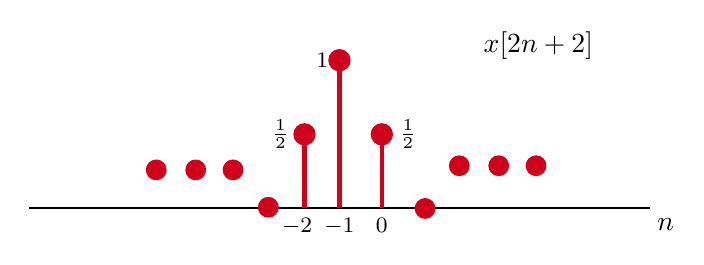
\begin{tikzpicture}[x=0.75pt,y=0.75pt,yscale=-1,xscale=1]
%uncomment if require: \path (0,364); %set diagram left start at 0, and has height of 364

%Straight Lines [id:da06072638558515686] 
\draw    (378.71,168) -- (79.29,168) ;
%Straight Lines [id:da5547538617459793] 
\draw [color={rgb, 255:red, 208; green, 2; blue, 27 }  ,draw opacity=1 ][fill={rgb, 255:red, 208; green, 2; blue, 27 }  ,fill opacity=1 ][line width=1.5]    (229,96.58) -- (229,168) ;
\draw [shift={(229,96.58)}, rotate = 90] [color={rgb, 255:red, 208; green, 2; blue, 27 }  ,draw opacity=1 ][fill={rgb, 255:red, 208; green, 2; blue, 27 }  ,fill opacity=1 ][line width=1.5]      (0, 0) circle [x radius= 4.36, y radius= 4.36]   ;
%Straight Lines [id:da8545689410720038] 
\draw [color={rgb, 255:red, 208; green, 2; blue, 27 }  ,draw opacity=1 ][fill={rgb, 255:red, 208; green, 2; blue, 27 }  ,fill opacity=1 ][line width=1.5]    (249.42,132.29) -- (249.42,167.71) ;
\draw [shift={(249.42,132.29)}, rotate = 90] [color={rgb, 255:red, 208; green, 2; blue, 27 }  ,draw opacity=1 ][fill={rgb, 255:red, 208; green, 2; blue, 27 }  ,fill opacity=1 ][line width=1.5]      (0, 0) circle [x radius= 4.36, y radius= 4.36]   ;
%Straight Lines [id:da9437858155461635] 
\draw [color={rgb, 255:red, 208; green, 2; blue, 27 }  ,draw opacity=1 ][fill={rgb, 255:red, 208; green, 2; blue, 27 }  ,fill opacity=1 ][line width=1.5]    (212.16,132.29) -- (212.16,167.71) ;
\draw [shift={(212.16,132.29)}, rotate = 90] [color={rgb, 255:red, 208; green, 2; blue, 27 }  ,draw opacity=1 ][fill={rgb, 255:red, 208; green, 2; blue, 27 }  ,fill opacity=1 ][line width=1.5]      (0, 0) circle [x radius= 4.36, y radius= 4.36]   ;
%Shape: Circle [id:dp8415745106048833] 
\draw  [color={rgb, 255:red, 208; green, 2; blue, 27 }  ,draw opacity=1 ][fill={rgb, 255:red, 208; green, 2; blue, 27 }  ,fill opacity=1 ] (190.24,167.42) .. controls (190.24,164.94) and (192.25,162.92) .. (194.74,162.92) .. controls (197.22,162.92) and (199.24,164.94) .. (199.24,167.42) .. controls (199.24,169.91) and (197.22,171.92) .. (194.74,171.92) .. controls (192.25,171.92) and (190.24,169.91) .. (190.24,167.42) -- cycle ;
%Shape: Circle [id:dp1924487381459985] 
\draw  [color={rgb, 255:red, 208; green, 2; blue, 27 }  ,draw opacity=1 ][fill={rgb, 255:red, 208; green, 2; blue, 27 }  ,fill opacity=1 ] (265.76,168) .. controls (265.76,165.51) and (267.78,163.5) .. (270.26,163.5) .. controls (272.75,163.5) and (274.76,165.51) .. (274.76,168) .. controls (274.76,170.49) and (272.75,172.5) .. (270.26,172.5) .. controls (267.78,172.5) and (265.76,170.49) .. (265.76,168) -- cycle ;
%Shape: Circle [id:dp9724739272897065] 
\draw  [color={rgb, 255:red, 208; green, 2; blue, 27 }  ,draw opacity=1 ][fill={rgb, 255:red, 208; green, 2; blue, 27 }  ,fill opacity=1 ] (173.24,149.42) .. controls (173.24,146.94) and (175.25,144.92) .. (177.74,144.92) .. controls (180.22,144.92) and (182.24,146.94) .. (182.24,149.42) .. controls (182.24,151.91) and (180.22,153.92) .. (177.74,153.92) .. controls (175.25,153.92) and (173.24,151.91) .. (173.24,149.42) -- cycle ;
%Shape: Circle [id:dp37116477968769124] 
\draw  [color={rgb, 255:red, 208; green, 2; blue, 27 }  ,draw opacity=1 ][fill={rgb, 255:red, 208; green, 2; blue, 27 }  ,fill opacity=1 ] (155.24,149.42) .. controls (155.24,146.94) and (157.25,144.92) .. (159.74,144.92) .. controls (162.22,144.92) and (164.24,146.94) .. (164.24,149.42) .. controls (164.24,151.91) and (162.22,153.92) .. (159.74,153.92) .. controls (157.25,153.92) and (155.24,151.91) .. (155.24,149.42) -- cycle ;
%Shape: Circle [id:dp0005769558109711692] 
\draw  [color={rgb, 255:red, 208; green, 2; blue, 27 }  ,draw opacity=1 ][fill={rgb, 255:red, 208; green, 2; blue, 27 }  ,fill opacity=1 ] (136.24,149.42) .. controls (136.24,146.94) and (138.25,144.92) .. (140.74,144.92) .. controls (143.22,144.92) and (145.24,146.94) .. (145.24,149.42) .. controls (145.24,151.91) and (143.22,153.92) .. (140.74,153.92) .. controls (138.25,153.92) and (136.24,151.91) .. (136.24,149.42) -- cycle ;
%Shape: Circle [id:dp5765900568262574] 
\draw  [color={rgb, 255:red, 208; green, 2; blue, 27 }  ,draw opacity=1 ][fill={rgb, 255:red, 208; green, 2; blue, 27 }  ,fill opacity=1 ] (319.24,147.42) .. controls (319.24,144.94) and (321.25,142.92) .. (323.74,142.92) .. controls (326.22,142.92) and (328.24,144.94) .. (328.24,147.42) .. controls (328.24,149.91) and (326.22,151.92) .. (323.74,151.92) .. controls (321.25,151.92) and (319.24,149.91) .. (319.24,147.42) -- cycle ;
%Shape: Circle [id:dp3702216225275915] 
\draw  [color={rgb, 255:red, 208; green, 2; blue, 27 }  ,draw opacity=1 ][fill={rgb, 255:red, 208; green, 2; blue, 27 }  ,fill opacity=1 ] (301.24,147.42) .. controls (301.24,144.94) and (303.25,142.92) .. (305.74,142.92) .. controls (308.22,142.92) and (310.24,144.94) .. (310.24,147.42) .. controls (310.24,149.91) and (308.22,151.92) .. (305.74,151.92) .. controls (303.25,151.92) and (301.24,149.91) .. (301.24,147.42) -- cycle ;
%Shape: Circle [id:dp5762492676349926] 
\draw  [color={rgb, 255:red, 208; green, 2; blue, 27 }  ,draw opacity=1 ][fill={rgb, 255:red, 208; green, 2; blue, 27 }  ,fill opacity=1 ] (282.24,147.42) .. controls (282.24,144.94) and (284.25,142.92) .. (286.74,142.92) .. controls (289.22,142.92) and (291.24,144.94) .. (291.24,147.42) .. controls (291.24,149.91) and (289.22,151.92) .. (286.74,151.92) .. controls (284.25,151.92) and (282.24,149.91) .. (282.24,147.42) -- cycle ;

% Text Node
\draw (380.71,171.4) node [anchor=north west][inner sep=0.75pt]    {$n$};
% Text Node
\draw (206.16,132.29) node [anchor=east] [inner sep=0.75pt]  [font=\footnotesize]  {$\frac{1}{2}$};
% Text Node
\draw (256.42,132.29) node [anchor=west] [inner sep=0.75pt]  [font=\footnotesize]  {$\frac{1}{2}$};
% Text Node
\draw (225,96.58) node [anchor=east] [inner sep=0.75pt]  [font=\footnotesize]  {$1$};
% Text Node
\draw (208.58,171.4) node [anchor=north] [inner sep=0.75pt]  [font=\footnotesize]  {$-2$};
% Text Node
\draw (229,171.4) node [anchor=north] [inner sep=0.75pt]  [font=\footnotesize]  {$-1$};
% Text Node
\draw (249.42,171.4) node [anchor=north] [inner sep=0.75pt]  [font=\footnotesize]  {$0$};
% Text Node
\draw (297,81.4) node [anchor=north west][inner sep=0.75pt]    {$x[ 2n+2]$};


\end{tikzpicture}
